\documentclass{article}
\usepackage[utf8]{inputenc}
\usepackage{graphicx}
\title{Homework 2 Part 2}
\author{tdhammond }
\date{September 2021}

\begin{document}

\maketitle

6(b): Using the grammar in Example 3.2, show a parse tree and a leftmost derivation for each of the following statements:
b. B = C * (A * C + B)\\
assign = $<$id$>$ = $<$expr$>$\\
	  B = $<$expr$>$\\
	  B = $<$id$>$ * $<$expr$>$\\
	  B = C * $<$expr$>$\\
	  B = C * ($<$expr$>$)\\
	  B = C * ($<$id$>$ * $<$expr$>$)\\
	  B = C * (A * $<$expr$>$)\\
	  B = C * (A * $<$id$>$ + $<$expr$>$)\\
	  B = C * (A * C + $<$expr$>$)\\
	  B = C * (A * C + B)\\
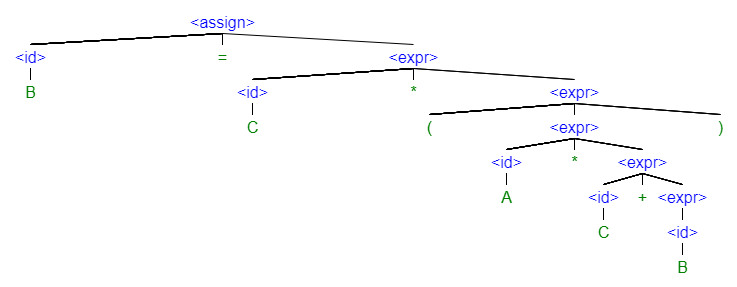
\includegraphics[scale=.5]{6b.png} \\

12: Consider the following grammar:\\
$<$S$>$ $\rightarrow$ a $<$S$>$ c $<$B$>$ $|$ $<$A$>$ $|$ b\\
$<$A$>$ $\rightarrow$ c $<$A$>$ $|$ c\\
$<$B$>$ $\rightarrow$ d $|$ $<$A$>$\\
Which of the following sentences are in the language generated by this grammar?\\
a. abcd\\
b. acccbd\\
c. acccbcc\\
d. acd\\
e. accc\\

A. abcd\\
$<$S$>$\\
a $<$S$>$ c $<$B$>$ $|$ $<$S$>$ $\rightarrow$ a $<$S$>$ c $<$B$>$\\
a b c $<$B$>$ $|$ $<$S$>$ $\rightarrow$ b\\
a b c d $|$ $<$B$>$ $\rightarrow$ d\\

E. accc\\
$<$S$>$\\
a $<$S$>$ c $<$B$>$ $|$ $<$S$>$ $\rightarrow$ a $<$S$>$ c $<$B$>$\\
a $<$A$>$ c $<$B$>$ $|$ $<$S$>$ $\rightarrow$ $<$A$>$\\
a c c $<$B$>$ $|$ $<$A$>$ $\rightarrow$ c\\
a c c $<$A$>$ $|$ $<$B$>$ $\rightarrow$ $<$A$>$\\
a c c c $|$ $<$A$>$ $\rightarrow$ c\\

18. What is the difference between an intrinsic attribute and a non-intrinsic
synthesized attribute? Intrinsic attributes are synthesized attributes of leaf nodes whose values are determined outside the parse tree. The value of a non-intrinsic synthesized attribute on a parse tree node depends only on the values of the attributes on that node's children nodes.\\

21e. . Using the virtual machine instructions given in Section 3.5.1.1, give an
operational semantic definition of the following: e. C switch
\\
\\switch(expr)\\
\indent case1:\\
\indent \indent stmt1;\\
\indent \indent break;\\
    \\
\indent default:\\
\indent \indent stmt2;\\

22e. Write a denotational semantics mapping function for the following
statements: e. C switch \\

28.Prove the following program is correct:\\
$\{n > 0\}$\\
count = n;\\
sum = 0;\\
while count $<>$ 0 do\\
sum = sum + count;\\
count = count - 1;\\
end\\
\{sum = 1 + 2 + . . . + n\}\\




\end{document}
